%!TEX root = ./main.tex

\section{Introduction}

% Introduction and motivation for our problem
% main objective: compare the best combination of experts.
% So for in the literature, always compare to the best expert (ex., regret)

The domain of algorithms with predictions (or learning-augmented algorithms \citep{MitzenmacherVassilvitskii20:Beyond-the-Worst-Case}) emerged recently and grew immensely at the intersection of (discrete) algorithm design and machine learning (ML).
Combining ML techniques with traditional algorithm design methods enables online algorithms to benefit from predictions that can infer future information from patterns in past data. Online algorithms with predictions can obtain performance guarantees beyond the worst-case analysis and provide fine-tuned solutions to various problems. In the literature, many significant problems have new learning-augmented results, for example, scheduling \citep{LattanziLavastida20:Online-scheduling,Mitzenmacher20:Scheduling-with}, paging \citep{LykourisVassilvtiskii18:Competitive-caching,Rohatgi20:Near-optimal-bounds,AntoniadisCoester20:Online-metric}, ski rental \citep{GollapudiPanigrahi19:Online-algorithms,KumarPurohit18:Improving-online,AngelopoulosDurr20:Online-Computation}, counting sketches \citep{HsuIndyk19:Learning-Based-Frequency}, bloom filters \citep{KraskaBeutel18:The-case-for-learned,Mitzenmacher18:A-model-for-learned}, and metrical task systems \citep{AntoniosEtAll23:mixing-predictions-metric-algorithms}.

Even though predictions provide a glimpse of the future, there is no mathematical guarantee for their accuracy. Adjusting the algorithm's trust in the predictions is a significant challenge since online algorithms must make irrevocable decisions at each time step. Ideally, if the predictions are accurate, the algorithm should perform well compared to the offline setting. In contrast, if the predictions are misleading, the algorithm should maintain a competitive solution, similar to the online setting where no predictive information is available. In other words, online algorithms with predictions are expected to bring the best of both worlds: mathematical performance guarantees of classical algorithms and good future prediction capabilities of machine learning methods.

Predictions can come from multiple sources (for example: heuristics, oracles, and randomized methods), but we ignore their nature and call all of them \emph{experts}.  An algorithm's consistency with the experts' suggestions is typically measured by comparing the algorithm's result with the solution of the \emph{best} expert. A representative example is the popular notion of regret in online learning, which fueled the development of many powerful algorithms and techniques.

A natural research question is whether it is possible to design competitive algorithms with mathematical performance guarantees with a stronger benchmark than the best expert. Comparing an algorithm with a stronger benchmark could provide deeper insights into the learning process and give better ways of exploiting the experts' predictions.

Taking a broader view, we can study whether combining predictions of several experts is similar to combining multiple online algorithms and whether we can expect to achieve better solutions with the combination. Assuming that we do not know in advance which of the given algorithms would perform best on the upcoming requests, can we combine the algorithms in some generic way to obtain a competitive online strategy? This has been a long-standing question in the community of online algorithms \citep{AzarBroder93:On-line-Choice,BlumBurch00:On-line-Learning}. To find an answer, it is a crucial to understand to what extent an online strategy can benefit from the input of multiple algorithms and which benchmark suits to evaluate its performance.

While in a completely general setting, such an online strategy and a corresponding benchmark may not exist, in this paper we propose
two algorithms for online linear and non-linear problems with covering constraints that are competitive with the new benchmark (the \emph{best linear combination} of the experts). Thus, our paper partially addresses the question we raised in the previous paragraph.

\subsection{Model and Problem}

\paragraph{Covering problem with experts.}
In the \emph{linear} problem setting, we have $n$ resources, and each resource $i$ has a cost per unit $c_{i}$ that we know in advance ($1 \leq i \leq n$).
Let $x_{i}$ be a non-negative variable representing the amount chosen from resource $i$.
The total cost of a solution is $\sum_{i=1}^{n} c_{i} x_{i}$.
The problem includes $K$ experts, and the problem's covering-type constraints are revealed online one by one.
At each time $t \geq 1$, we receive a covering constraint $\sum_{i=1}^{n} a_{i}^{t} x_{i} \geq 1$ (where $a_{i}^{t} \geq 0$) and each expert $k$ provides
a solution $(s_{i,k}^{t})_{i=1}^{n}$. Our algorithm can observe the experts' solutions, and afterwards, it must update its own solution (denoted as $(x_{i}^{t})_{i=1}^{n}$)
to satisfy the new constraint while maintaining the satisfaction of the previous ones. This algorithm must update its solution in the sense of online algorithms, formally, $x_{i}^{t} \geq x_{i}^{t-1} ~\forall\ i, t$.
Our goal is to design an algorithm that minimizes $\sum_{i=1}^{n} c_{i} x_{i}^{T}$ subject to
all online covering constraints $t$, where $1 \leq t \leq T$. The value $T$ is the last time a constraint is released, and it is not known by the algorithm.

The \emph{non-linear} problem setting is analogous to the linear one, since we consider non-linear problems with linear constraints. However, the total cost of the solution $(x_{i}^t)_{i=1}^{n}$, becomes $f(x^t)$, where $f$ is a non-linear function. This setting captures different classes of problems: online mixed packing and covering, submodular optimization, etc.

\noindent \textbf{Experts.} \label{subsec:experts} In our model, the experts' predictions are also \emph{online solutions} fulfilling these properties:
\begin{compactenum}
	\item for every expert $k$ and for every time $t$ the solution $(s_{i,k}^{t})_{i=1}^{n}$ is feasible, therefore, every constraint $t'$ where $1 \leq t' \leq t$ is satisfied;
	\item for every expert $k$ and for every time $t$ and for every resource $i$, the previous expert solutions are irrevocable, therefore $s_{i,k}^{t} \geq s_{i,k}^{t'}$ for all $t' \leq t$.
\end{compactenum}
These properties can be verified online. If some experts do not satisfy them, we simply ignore those experts both in the decision-making and in the benchmark.
We provide motivations and justification for the assumptions in \cref{sec:assumptions}.

%A crucial remark: we do \emph{not} assume that the experts' solutions are tight at each constraint $t$, requiring $\sum_{i=1}^{n} a_{i}^{t} s_{i,k}^{t} = 1 ~ \forall t, k$ to hold.
%This assumption is unrealistic and cannot be maintained in an online manner (see the discussion in Appendix~\ref{appix-tight-solutions}).
%Besides, assuming tight constraint satisfaction would simplify the problem, while intuitively,
%the difficulty of designing competitive algorithms comes from the lack of obvious ways to distinguish
%good expert solutions from (probably many) non-efficient/misleading ones.

\noindent \textbf{Benchmark.}
We consider a dynamic benchmark that captures the \emph{best linear combination} of all experts' solutions \emph{over time}.
Informally, at any online time step, the benchmark can take a linear combination of the experts' solutions.
The linear combination can be \emph{dynamically} changed over time, and it can be different from previous combinations.
However, the benchmark's decisions are also online, so it cannot decrease the value of the decision variables ($x_{i}$).
We refer to our benchmark with the name \texttt{LIN-COMB} from now on.

%\begin{wrapfigure}{r}{0.7\textwidth}
\begin{figure}
	\vspace{-0.5cm}
	\begin{mdframed}
	\vspace{-0.2cm}
		\begin{align*}
			\text{Linear:}  \qquad \min \sum_{i=1}^{n} c_{i} x_{i}^{T} &= \sum_{i=1}^{n} c_{i} \sum_{t=1}^{T}\bigl( x_{i}^{t} - x_{i}^{t-1}\bigr) & \\
			\text{Non-linear:} \qquad \min f(x^{T}) \hspace{0.37cm} & & \\
			\text{s.t.} \hspace{1.63cm}
			\sum_{k=1}^{K} w_{k}^{t} &= 1 \qquad &\forall t \\
			%
			\qquad x_{i}^{t} &\geq \sum_{k=1}^{K} w_{k}^{t} s_{i,k}^{t}  \qquad &\forall i, t\\
			%
			\qquad x_{i}^{t} &\geq x_{i}^{t-1} \qquad &\forall i, t \\
			%
			\qquad w_{k}^{t} &\geq 0 \qquad &\forall t, k
		\end{align*}
		%where $1 \leq t \leq T$, $1 \leq i \leq n$, and $f$ is non-linear.
	\end{mdframed}
	\vspace{-0.2cm}
	\caption{\texttt{LIN-COMB} benchmark}
	\label{fig:benchmark}
	\vspace{-0.5cm}
\end{figure}
%\end{wrapfigure}

The \texttt{LIN-COMB} benchmark's formal description is visible on \cref{fig:benchmark}.
Let $w_{k}^{t} \geq 0$ be the weight assigned by the \texttt{LIN-COMB} benchmark to expert $k$ (where $1 \leq k \leq K$) at time
$1 \leq t \leq T$.
Since we consider a linear combination, the constraint $ \sum_{k=1}^{K} w_{k}^{t} = 1$ must hold.
%In the linear program, we consider the relaxed version of this constraint, where $\sum_{k=1}^{K} w_{k}^{t} \geq 1$.
The solution of \texttt{LIN-COMB} at time $t$ is ideally $x_{i}^{t} = \sum_{k=1}^{K} w_{k}^{t} s_{i,k}^{t}$,
however, $x_{i}^{t}$ must be larger than $x_{i}^{t-1}$.
Therefore, we set $x_{i}^{t} = \max\bigl\{\sum_{k=1}^{K} w_{k}^{t} s_{i,k}^{t},\ x_{i}^{t-1}\bigr\}$ for $1 \leq i \leq n$.
%


Since every expert's solution is feasible by our assumptions, at each time $t$ and for all resource~$i$,
the constructed solution $x_{i}^{t} \geq \sum_{k=1}^{K} w_{k}^{t} s_{i,k}^{t}$ constitutes a feasible solution to the covering constraints of the original covering problem. Formally, for every constraint $t'$ with $t' \leq t$,
%
\begin{align*}
	\sum_{i=1}^{n} a_{i}^{t'} x_{i}^{t} &\geq
	%
	\sum_{i=1}^{n} a_{i}^{t'} \biggl( \sum_{k=1}^{K} w_{k}^{t} s_{i,k}^{t} \biggr)
	%
	= \sum_{k=1}^{K} w_{k}^{t}  \biggl( \sum_{i=1}^{n} a_{i}^{t'} s_{i,k}^{t} \biggr)
	%
	 \geq \sum_{k=1}^{K} w_{k}^{t} \geq 1
\end{align*}
%
where the second inequality holds due to the feasibility of the experts' solutions.
%

We highlight that the best-expert benchmark is included in \texttt{LIN-COMB}.
We get the solution of this benchmark by setting $w^{t}_{k^{*}} = 1$ for all $t$, where $1 \leq t \leq T$, and $w^{t}_{k} = 0$ for all $k \neq k^{*}$,
where $k^{*}$ is the best expert (so $x_{i}^{t} = s_{i,k^{*}}^{t}$ for all $i$ and $t$).
Indeed, compared to the best expert in hindsight, \texttt{LIN-COMB} is equivalent in the linear setting and
is stronger in a more general non-linear setting. For a detailed discussion see \cref{sec:comparaison}. Here, we briefly provide an example with non-linear objectives.
Consider the makespan minimization problem in which one assigns $n$ unit jobs to $n$ identical machines to minimize the maximum machine load.
There are $n$ experts and each expert~$i$ assigns all jobs to machine~$i$. Hence, the best expert has the maximum machine load of $n$ (the same for every expert). However, the optimal solution in \texttt{LIN-COMB} can choose $w_{i} = 1/n$, which results in the makespan of $1$. The solution corresponds to the assignment of one job to one machine.

\subsection{Our approach and contribution}

\paragraph{Approach.} We rely on the primal-dual approach in our algorithm design. To lower bound the algorithm's objective value, we relax the linear program formulation of \texttt{LIN-COMB}. Then, we take the dual of the relaxation, which is a lower bound on the relaxation. Following the chain of lower bounds, the dual problem is a lower bound on the original \texttt{LIN-COMB} benchmark.
%The formulations of the relaxation and its dual are detailed in \cref{sec:covering} for linear problems and in \cref{sec:convex} for non-linear problems. \textbf{\color{red} to change here }

Both of our proposed algorithms set the decision variables at every time step based on the solution of an internal program. Our approach is inspired by the
convex regularization method of \cite{BuchbinderChen14:Competitive-Analysis}.
When the objective cost is a linear function, it is well-known that the regularization function is a shifted entropy function.
These functions have been widely used, in particular in the recent breakthrough related to $k$-server \citep{BubeckCohen18:K-server-via-multiscale,BuchbinderGupta19:k-servers-with}
and metrical task system problems \citep{BubeckCohen21:Metrical-task},
in which the entropy functions are shifted by constant parameters.

A novel point in our approach is that the entropy function is shifted by the average of the experts' solutions.
Moreover, regarding the constraints of the internal program, instead of using the experts' solutions directly,
we define auxiliary solutions that guarantee tight constraint satisfaction.
Intuitively, this step is useful to avoid misleading experts' suggestions.

It is more challenging to find a regularization function for non-linear objective functions.
In our approach, we propose a new regularizer by coupling the entropy-like function with the gradient-Lipschitz property of the original covering problem's objective function.
This new regularization function allows us to analyze the non-linear objective setting similarly to the linear case.

\paragraph{Results.} Let $\rho$ be the maximum ratio between the experts' solutions on the resources.
Informally, $\rho$ represents the discrepancy across the experts' predictions.
Formally,
%We define the following parameter to establish the competitive ratio of our algorithm.
\[
	\rho := \max_{i} \max_{t',t''} \biggl\{\frac{\sum_{k=1}^{K} s_{i,k}^{t'}}{\sum_{k=1}^{K} s_{i,k}^{t''}} \biggr\}  \textnormal{ s.t. } \sum_{k=1}^{K} s_{i,k}^{t''} > 0.
\]

Our main results are the following.
First, we present an algorithm for the online linear covering problem that achieves an objective cost at most $O(\ln(K\rho))$ times the cost of the \texttt{LIN-COMB} benchmark.
For the online non-linear covering problem, we provide an algorithm that achieves an objective cost at most $O(\ln(K\rho)) \cdot \frac{\lambda}{(1-\mu\ln(K\rho))}$ times the cost of \texttt{LIN-COMB}, where ($\lambda$,$\mu$) are parameters of the non-linear objective function (precisely, ($\lambda$,$\mu$) are smoothness parameters of the objective function that we define later in the corresponding section).

In particular, for $0$-$1$ optimization problems, where the experts provide integer (deterministic or randomized) solutions, our first algorithm is $O(\ln(K))$-competitive with \texttt{LIN-COMB}, and the second one is $O(\ln(K)) \cdot \frac{\lambda}{(1-\mu\ln(K))}$-competitive.
Remarkably, our algorithms are resilient against the prediction quality fluctuations (discussion in \cref{subsec:related-works} and experiments in \cref{sec:exp}).


\subsection{Related work and discussions} \label{subsec:related-works}

Much of the research focusing on surpassing worst-case performance guarantees is motivated by the spectacular advances of machine learning (ML). Specifically, ML methods can detect patterns among the arriving input requests and provide valuable insights for the online algorithms regarding future requests. \cite{LykourisVassilvtiskii18:Competitive-caching} introduced a general framework to integrate ML predictions into classical algorithm designs to surpass the worst-case performance limit.
As a result, many practically relevant online problems were revisited to enhance existing classical algorithms with ML predictions (see the aforementioned \citep{LattanziLavastida20:Online-scheduling,Mitzenmacher20:Scheduling-with,LykourisVassilvtiskii18:Competitive-caching,Rohatgi20:Near-optimal-bounds,AntoniadisCoester20:Online-metric,GollapudiPanigrahi19:Online-algorithms,KumarPurohit18:Improving-online,AngelopoulosDurr20:Online-Computation,HsuIndyk19:Learning-Based-Frequency,KraskaBeutel18:The-case-for-learned,Mitzenmacher18:A-model-for-learned,AntoniosEtAll23:mixing-predictions-metric-algorithms}).

On a high-level view, we aim to design algorithms that are robust (competitive) to the offline optimal solution and also consistent with the expert's predictions. Ideally, the performance of the designed algorithm should surpass previous bounds whenever the predictions are reliable (low errors).
However, most learning-augmented algorithms suffer when the error rates are neither very low nor very high, resulting in prediction confidence that is neither very low nor very high.
Figure~\ref{fig:robustness-consistency} provides a general picture of the performance of an algorithm with predictions, which is representative for many problems (for example, \cite{BamasMaggoriSvensson20:primal-dual-method,KeviNguyen23:Primal-Dual-Algorithms}).

\begin{wrapfigure}{r}{0.43\textwidth}
	\vspace{-0.6cm}
    \centering
    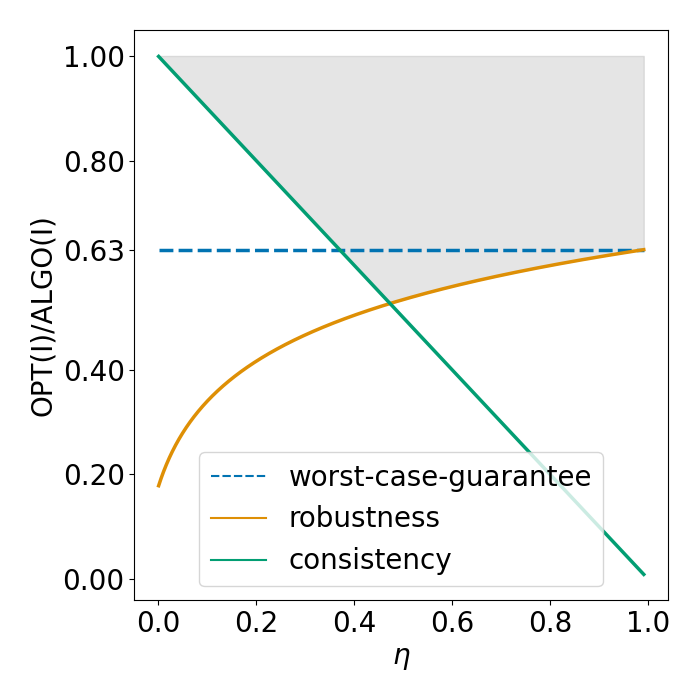
\includegraphics[width=0.45\textwidth]{./Img/consistency_robustness.png}
    \vspace{-0.8cm}
    \caption{Robustness-Consistency}
    \label{fig:robustness-consistency}
    \vspace{-0.3cm}
\end{wrapfigure}

In the figure, $\eta$ indicates the confidence in the predictions (or equivalently the error rate of predictions). The learning-augmented algorithm's performance bound is the maximum value of the green and orange curves (gray shaded area on the figure). We can observe that when $0.4 \leq \eta \leq 0.9$,
the algorithm's performance guarantee is worse than the classical worst-case guarantee.
Intuitively, in the case of neither very low nor very high confidence in the predictions, the algorithm has a hard time deciding which component it should follow.
It raises the question whether we can achieve at least a constant factor of the worst-case guarantee (where the constant is as close to 1 as possible) while assuring a resilient output solution regardless of the predictions' quality.
Our algorithms with the new benchmark provide an answer to this question.






%The paper of \cite{AnandGe22:Online-Algorithms} is the closest to ours, which also studies the design of algorithms with multiple experts.
%They consider a \texttt{DYNAMIC} benchmark that is intuitively
%the minimum cost solution that is supported by at least one expert solution at each time step. Formally:
%\[\texttt{DYNAMIC} = \min_{\hat{\textbf{x}} \in \hat{X}} \sum_{i=1}^{n} c_i \hat{x}_i \textnormal{, where}\]
%%
%$\hat{X} = \{\hat{\vect{x}} : \forall\ i \in [n],\ \forall\ t \in [T],\ \exists\ k \in [K]\ \textnormal{ s.t. } s_{i,k}^{t} \le \hat{x}_i \}$.
%%
%Our benchmark, \texttt{LIN-COMB}, is included in \texttt{DYNAMIC}, since every solution $x_{i}^{t}$ in \texttt{LIN-COMB} satisfies:
%$
%	x_{i}^{t} \geq \sum_{k=1}^{K} s_{i,k}^{t}w_{k}^{t} \geq \min_{k} \{s_{i,k}^{t}\}
%$.
%So for any $i$ and $t$, there exists $k$ such that $x_{i}^{t} \geq s_{i,k}^{t}$.
%However, the inverse is not true: a solution $\hat{\vect{x}}^{t} \in \hat{X}$ in \texttt{DYNAMIC} is not necessarily
%a linear combination of the experts' solutions.
%The \texttt{DYNAMIC} benchmark in \cite{AnandGe22:Online-Algorithms} relied on the assumption that at every time step
%the experts' solutions are tight. This assumption does not allow the representation of some realistic problems and it is impossible to maintain in online solutions (see Appendix~\ref{appix-tight-solutions}).
%Further, \cite{AnandGe22:Online-Algorithms} claimed an $O(\ln(K))$-competitive algorithm in the \texttt{DYNAMIC} benchmark.
%Unfortunately, their benchmark is too strong; we show an example in Appendix~\ref{sec:counter-example}
%in which their algorithm's performance guarantee is unbounded in their \texttt{DYNAMIC}
%benchmark. We believe that with a different benchmark their algorithm could be $O(\ln(K))$-competitive; however, we did not manage to prove this.


Integrating multiple predictions into online algorithms have been actively studied.
\cite{GollapudiPanigrahi19:skirental-multiple-predictions} studied the ski rental problem with multiple predictions.
The authors defined a consistency metric, which compares the performance of their algorithm to the optimal solution, given that at least one prediction (among the $k$ predictions) is optimal.
%By carefully integrating every prediction in their algorithm design, the authors managed to reduce the overall prediction error rate and obtain the best possible performance guarantee for their algorithm. During their analysis, they defined a consistency metric, which compares the performance of their algorithm to the optimal solution, given that at least one prediction (among the $k$ predictions) is correct.
\cite{AlmanzaChierichetti21:Online-Facility} also considered multiple predictions in the online facility location problem.
%The suggestions are treated as a family of sets and the authors use the union of these suggestions.
They compared the performance of their algorithm to the best possible solution obtained on the union of the suggestions. Recently, \cite{DinitzIm:Algorithms-with} studied the use of multiple predictors for several problems such as matching, load balancing, and non-clairvoyant scheduling. They provided algorithms that were competitive with the best predictor for such problems.
\cite{AnandGe22:Online-Algorithms} studies the design of algorithms with multiple experts for linear covering problems.
They consider a \texttt{DYNAMIC} benchmark that is intuitively
the minimum cost solution that is supported by at least one expert solution at each time step,
and provide an $O(\ln(K))$-competitive algorithm in the \texttt{DYNAMIC} benchmark.

%An important remark: all the above benchmarks are captured within \texttt{LIN-COMB}.

Furthermore, \cite{AntoniosEtAll23:mixing-predictions-metric-algorithms} proposed an algorithm with multiple experts for the metrical task system problem. Their benchmark allows switching from one expert to another at each time step, but it does not allow combinations of experts or any solution not suggested by one of the experts. In our \texttt{LIN-COMB} benchmark, the linear combination that evolves over time could result in a solution that is not suggested by any of the experts and potentially, it can be much more efficient. In \cite{AntoniosEtAll23:mixing-predictions-metric-algorithms} there is a cost for state transitions, which is appropriate in their setting, but in many other problems the smooth transition with additional costs from one state to another is not allowed (past decisions are immutable). Therefore, the results of \cite{AntoniosEtAll23:mixing-predictions-metric-algorithms} are not applicable to our setting.

Combining online algorithms into a new algorithm to achieve better results than the individual input algorithms has been a long-standing online algorithm design question \citep{AzarBroder93:On-line-Choice,BlumBurch00:On-line-Learning}.
Its intrinsic difficulty is similar to the issue we mentioned earlier: when the performance of the given input algorithms (or heuristics, randomized methods) is unclear (especially in the online setting), it is challenging to create a combination that can surpass the performance of the included algorithms.
Following the current development of online algorithm design techniques with multiple predictions, this subject has been renewed with different machine learning approaches. Our paper contributes to this line of research.

%\subsection{Paper overview}
%In this paper we show two algorithms to solve online \emph{linear} (\cref{sec:covering}) and online \emph{non-linear} (\cref{sec:convex}) covering problems with multiple experts.  \cref{sec:exp} shows empirical results, and we conclude in \cref{sec:conclusion}. The complete details can be found in the appendix.
